\documentclass[sigconf, nonacm, screen]{acmart}

%%
\usepackage{subcaption}
\usepackage{listings}
%%
\AtBeginDocument{
  \providecommand\BibTeX{{
    \normalfont B\kern-0.5em{\scshape i\kern-0.25em b}\kern-0.8em\TeX}}}

%%
\begin{document}

%%
\title{Design and Integration of an Accelerator for MRI with ESP}
\subtitle{Embedded Scalable Platforms (COMS E6868), Columbia University, Spring 2020}

%%
\author{Pei Liu}
\authornote{Project mentor: Davide Giri (davide.giri@columbia.edu). Instructor:
  Luca Carloni (luca@cs.columbia.edu).}
\email{pl2748@columbia.edu}
\affiliation{
  \institution{Department of Computer Science, Columbia University}
  \city{New York}
  \country{USA}
}

%%
\begin{abstract}
I plan to design an accelerator to calculate the Magnetic Resonance Imaging Q
matrix through SystemC and HLS tool Stratus and implement this design on
FPGA. Then I plan to explore the design space to get a thorough understanding of
the methodology of designing accelerators though ESP.
\end{abstract}

%%
\maketitle

\section{Introduction}
\label{sec:intro}

Magnetic Resonance Imaging is commonly used by the medical community for safe
and non-invasive probing of the structure and function of human bodies. Images
generated using MRI have a profound impact both in clinical and research
fields.\\
\\
MRI has a scan phase (data acquisition) and an image reconstruction phase. Short
scan time can increase scanner throughput and reduce patient discomfort, which
tends to mitigate motion-related artifacts. At the same time, high resolution of
the image is preferable, but it requires a longer scan time.
%
Sampling across a uniform grid (Cartesian trajectory sampling) enables quick and
efficient image reconstruction, but it requires a rather long scan time, which
limits the image resolution. Non-uniform sampling (non-Cartesian trajectory
sampling), instead, is faster and less sensitive to imaging artifacts, because
it incorporates some prior anatomical knowledge to scan specific areas with
higher resolution. However, this approach requires significantly more
computation for image reconstruction~\cite{stone2008accelerating}.\\
\\
This work focuses on the hardware acceleration of one key component of the image
reconstruction for non-Cartesian trajectory sampling: the computation of the Q
matrix~\cite{stratton2012parboil}. For this purpose we use ESP, a platform for
agile system-on-chip (SoC) design~\cite{esp-website, esp-release}. With ESP, we
design a hardware accelerator for the MRI-Q algorithm, we perform a design-space
exploration (DSE), and we integrate the accelerator in a full system-on-chip
(SoC). Finally, we evaluate the accelerator performance by prototyping the full
SoC on FPGA.

\section{Specifications}

\subsection{Reference Application}

The MRI-Q algorithm is shown in \figurename~\ref{fig:algo}. It is part of the
Parboil Benchmarks~\cite{stratton2012parboil}, and it corresponds to equation 3
in the MRI reconstruction paper by \emph{Stone et
  al.}~\cite{stone2008accelerating}.
%
As our reference application, we use the C implementation of the algorithm and
the input datasets provided as part of the Parboil benchmarks. The datasets are
listed in Table~\ref{tab:datasets}.


\begin{figure}[t]
\centering
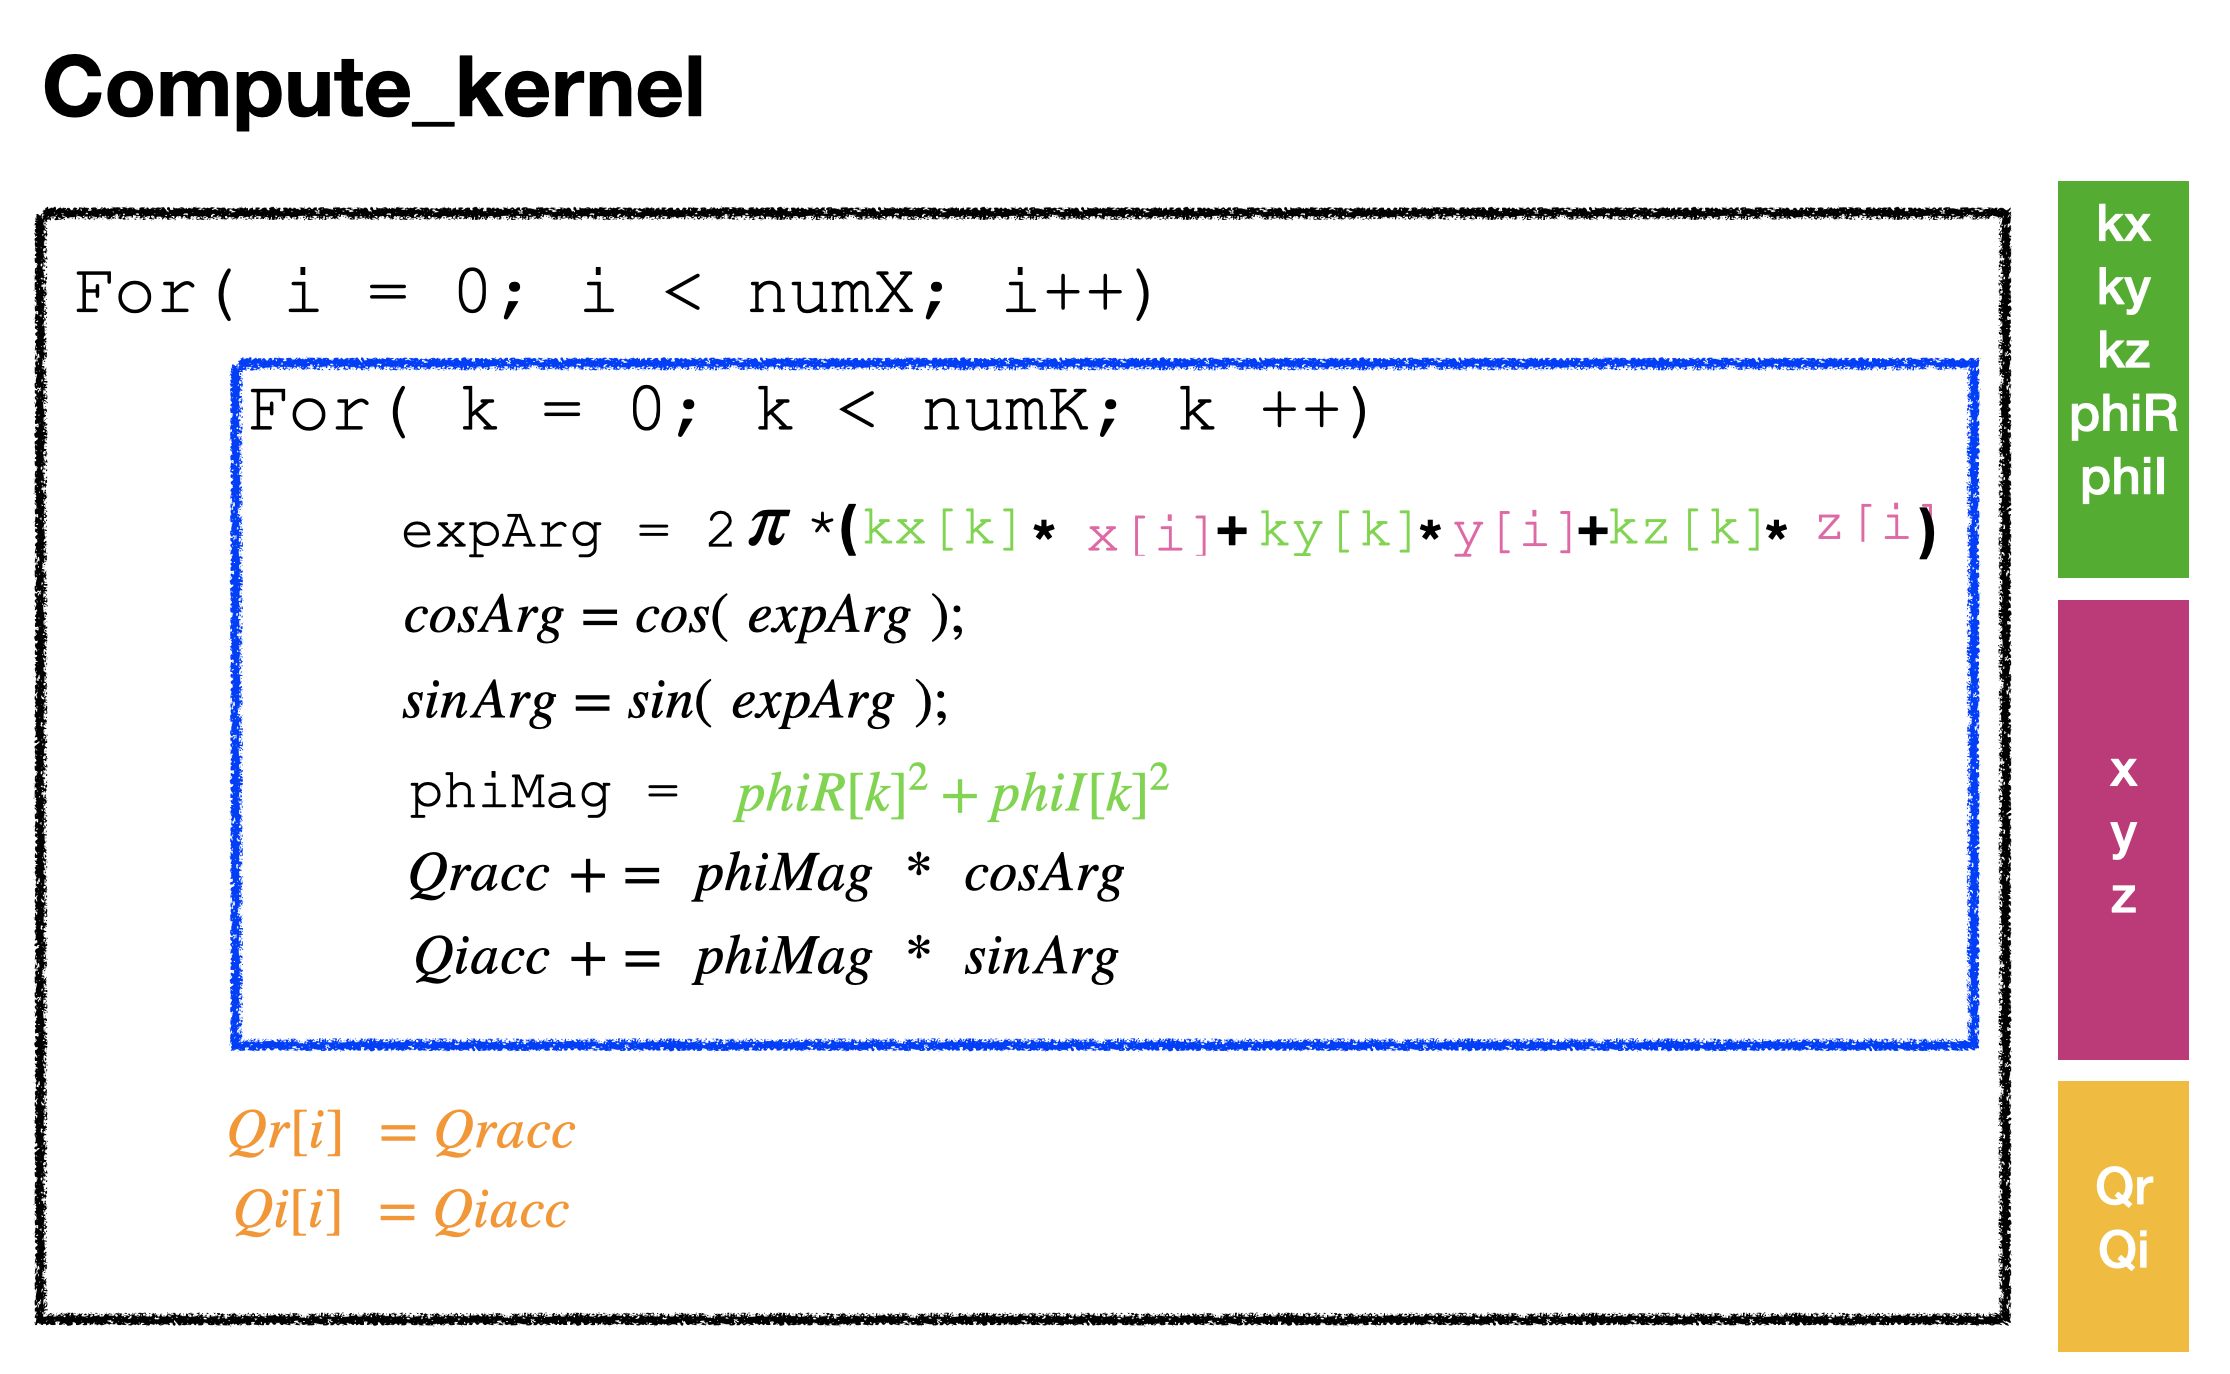
\includegraphics[width=\columnwidth]{figures/algorithm}
\caption{Algorithm for computing the MRI-Q matrix.}
\label{fig:algo}
\end{figure}


\begin{table}[t]
\centering
\begin{tabular}{c|c|c|c}
\toprule
\textbf{name} & \textbf{image size} & \textbf{\# of pixels} & \textbf{K-space dimension} \\
\midrule
small       & 32*32*32    & 32768   & 3072    \\
large       & 64*64*64    & 262144  & 2048    \\
128*128*128 & 128*128*128 & 2097152 & 2097152 \\
\bottomrule
\end{tabular}
\caption{Datasets for MRI-Q from Parboil Benchmarks.}
\label{tab:datasets}
\end{table}


\subsection{Accelerator and SoC Design}

We design an accelerator that can work with any input image size, including the
sizes of all three datasets in Table~\ref{tab:datasets}. We design the
accelerator in SystemC for Cadence Stratus HLS. As a starting point, we use the
ESP accelerator design flow to automatically generate a skeleton of accelerator,
testbench, test applications, and device driver.
%
We perform a DSE leveraging multiple HLS knobs to obtain
multiple implementation of the accelerator with different tradeoffs of area and
latency.
%
Then, with the ESP SoC design flow, we create multiple SoCs containing one
implementation of the accelerator and one processor core.

\subsection{Evaluation}

We will both validate and evaluate the accelerator in isolation with a SystemC
testbench (used for the simulation of both behavioral SystemC and HLS-generated
RTL), and as part of a full SoC with RTL simulation and FPGA prototyping. On the
full SoC we execute either bare-metal programs or Linux applications (FPGA
only).

The validation consists in verifying the correctness of the
accelerator output (the Q matrix) against the expected output computed by the
reference application.

To estimate performance and resources utilization we first use RTL simulation of
the HLS-generated RTL and the Stratus HLS reports. Then we measure the
accelerator performance on FPGA, and we collect the resource utilization
information from the Vivado reports. On FPGA we compare the execution time of
the accelerator with the time required for running the reference application on
the processor core in the ESP SoC. This comparison provides an estimate of the
accelerator speedup with respect to a software execution of the algorithm on a
CPU.

We collect performance estimates of different implementations of the
accelerator obtained with the DSE.

\subsection{Milestones}
\label{sec:milestones}

\begin{enumerate}

\item Project proposal (by Feb. 5).
  
\item Reference application (by Feb. 12).

\item ESP tutorials: \emph{``How to design a single-core SoC''}, and \emph{``How
  to design an accelerator in SystemC (Cadence Stratus HLS)''} (by Feb. 19).

\item Skeleton generation for accelerator and test apps (by Feb. 19)
  
\item Accelerator and test apps customization (by Mar. 11)

\item SoC evaluation with RTL simulation (by Mar. 18)

\item SoC evaluation with FPGA prototyping (by Mar. 25)
  
\item Midterm presentation and report (by Mar. 25)
 
\item DSE and optimization (by May 13)

\item Final presentation and report (by May 13)

\end{enumerate}


%%
%% \begin{acks}
%% Optional acks
%% \end{acks}

%%
\bibliographystyle{ACM-Reference-Format}
\bibliography{ref}

%%
%%\appendix
%%\section{section title}

\end{document}
\endinput
